\section{Proving equivalence of X25519 in C and Coq}
\label{sec:C-Coq}

In this section we prove the following theorem:
% In this section we outline the structure of our proofs of the following theorem:

\begin{informaltheorem}
The implementation of X25519 in TweetNaCl (\TNaCle{crypto_scalarmult}) matches
the specifications of RFC~7748~\cite{rfc7748} (\Coqe{RFC}).
\end{informaltheorem}

More formally:
\begin{lstlisting}[language=Coq]
Theorem body_crypto_scalarmult:
  (* VST boiler plate. *)
  semax_body
    (* Clight translation of TweetNaCl. *)
    Vprog
    (* Hoare triples for fct calls. *)
    Gprog
    (* fct we verify. *)
    f_crypto_scalarmult_curve25519_tweet
    (* Our Hoare triple, see below. *)
    crypto_scalarmult_spec.
\end{lstlisting}

% We first describe the global structure of our proof (\ref{subsec:proof-structure}).
Using our formalization of RFC~7748 (\sref{sec:Coq-RFC}) we specify the Hoare
triple before proving its correctness with the VST (\ref{subsec:with-VST}).
We provide an example of equivalence of operations over different number
representations (\ref{subsec:num-repr-rfc}). Then, we describe efficient techniques
used in some of our more complex proofs (\ref{subsec:inversions-reflections}).


\subsection{Applying the Verifiable Software Toolchain}
\label{subsec:with-VST}

We now turn our focus to the formal specification of \TNaCle{crypto_scalarmult}.
We use our definition of X25519 from the RFC in the Hoare triple and prove
its correctness.

\subheading{Specifications.}
We show the soundness of TweetNaCl by proving a correspondence between
the C version of TweetNaCl and the same code as a pure Coq function.
% why "pure" ?
% A pure function is a function where the return value is only determined by its
% input values, without observable side effects (Side effect are e.g. printing)
This defines the equivalence between the Clight representation and our Coq
definition of the ladder (\coqe{RFC}).

\begin{lstlisting}[language=CoqVST]
Definition crypto_scalarmult_spec :=
DECLARE _crypto_scalarmult_curve25519_tweet
WITH
  v_q: val, v_n: val, v_p: val, c121665:val,
  sh : share,
  q : list val, n : list Z, p : list Z
(*------------------------------------------*)
PRE [ _q OF (tptr tuchar),
     _n OF (tptr tuchar),
     _p OF (tptr tuchar) ]
PROP (writable_share sh;
      Forall (fun x => 0 <= x < 2^8) p;
      Forall (fun x => 0 <= x < 2^8) n;
      Zlength q = 32; Zlength n = 32;
      Zlength p = 32)
LOCAL(temp _q v_q; temp _n v_n; temp _p v_p;
      gvar __121665 c121665)
SEP  (sh [{ v_q }] <<(uch32)-- q;
      sh [{ v_n }] <<(uch32)-- mVI n;
      sh [{ v_p }] <<(uch32)-- mVI p;
      Ews [{ c121665 }] <<(lg16)-- mVI64 c_121665)
(*------------------------------------------*)
POST [ tint ]
PROP (Forall (fun x => 0 <= x < 2^8) (RFC n p);
      Zlength (RFC n p) = 32)
LOCAL(temp ret_temp (Vint Int.zero))
SEP  (sh [{ v_q }] <<(uch32)-- mVI (RFC n p);
      sh [{ v_n }] <<(uch32)-- mVI n;
      sh [{ v_p }] <<(uch32)-- mVI p;
      Ews [{ c121665 }] <<(lg16)-- mVI64 c_121665
\end{lstlisting}

In this specification we state preconditions like:
\begin{itemize}
  \item[] \VSTe{PRE}: \VSTe{_p OF (tptr tuchar)}\\
  The function \TNaCle{crypto_scalarmult} takes as input three pointers to
  arrays of unsigned bytes (\VSTe{tptr tuchar}) \VSTe{_p}, \VSTe{_q} and \VSTe{_n}.
  \item[] \VSTe{LOCAL}: \VSTe{temp _p v_p}\\
  Each pointer represent an address \VSTe{v_p},
  \VSTe{v_q} and \VSTe{v_n}.
  \item[] \VSTe{SEP}: \VSTe{sh [{ v_p $\!\!\}\!\!]\!\!\!$ <<(uch32)-- mVI p}\\
  In the memory share \texttt{sh}, the address \VSTe{v_p} points
  to a list of integer values \VSTe{mVI p}.
  \item[] \VSTe{PROP}: \VSTe{Forall (fun x => 0 <= x < 2^8) p}\\
  In order to consider all the possible inputs, we assume each
  element of the list \texttt{p} to be bounded by $0$ included and $2^8$
  excluded.
  \item[] \VSTe{PROP}: \VSTe{Zlength p = 32}\\
  We also assume that the length of the list \texttt{p} is 32. This defines the
  complete representation of \TNaCle{u8[32]}.
\end{itemize}

As postcondition we have conditions like:
\begin{itemize}
  \item[] \VSTe{POST}: \VSTe{tint}\\
  The function \TNaCle{crypto_scalarmult} returns an integer.
  \item[] \VSTe{LOCAL}: \VSTe{temp ret_temp (Vint Int.zero)}\\
  The returned integer has value $0$.
  \item[] \VSTe{SEP}: \VSTe{sh [{ v_q $\!\!\}\!\!]\!\!\!$ <<(uch32)-- mVI (RFC n p)}\\
  In the memory share \texttt{sh}, the address \VSTe{v_q} points
  to a list of integer values \VSTe{mVI (RFC n p)} where \VSTe{RFC n p} is the
  result of the \TNaCle{crypto_scalarmult} of \VSTe{n} and \VSTe{p}.
  \item[] \VSTe{PROP}: \VSTe{Forall (fun x => 0 <= x < 2^8) (RFC n p)}\\
  \VSTe{PROP}: \VSTe{Zlength (RFC n p) = 32}\\
  We show that the computation for \VSTe{RFC} fits in  \TNaCle{u8[32]}.
\end{itemize}

computes the same result as \VSTe{RFC} in Coq provided that inputs are within
their respective bounds: arrays of 32 bytes.

The correctness of this specification is formally proven in Coq with
\coqe{Theorem body_crypto_scalarmult}.

This specification (proven with VST) shows that \TNaCle{crypto_scalarmult} in C

% The Verifiable Software Toolchain uses a strongest postcondition strategy.
% The user must first write a formal specification of the function he wants to verify in Coq.
% This should be as close as possible to the C implementation behavior.
% This will simplify the proof and help with stepping through the Clight version of the software.
% With the range of inputs defined, VST mechanically steps through each instruction
% and ask the user to verify auxiliary goals such as array bound access, or absence of overflows/underflows.
% We call this specification a low level specification. A user will then have an easier
% time to prove that his low level specification matches a simpler higher level one.

% In order to further speed-up the verification process, it has to be know that to
% prove the specification \TNaCle{crypto_scalarmult}, a user only need the specification of e.g. \TNaCle{M}.
% This provide with multiple advantages: the verification by the Coq kernel can be done
% in parallel and multiple users can work on proving different functions at the same time.
% For the sake of completeness we proved all intermediate functions.

\subheading{Memory aliasing.}
%
The semicolon in the \VSTe{SEP} parts of the Hoare triples represents the \emph{separating conjunction} (often written as a star), which means that
the memory shares of \texttt{q}, \texttt{n} and \texttt{p} do not overlap.
In other words,
we only prove correctness of \TNaCle{crypto_scalarmult} when it is called without aliasing.
But for other TweetNaCl functions, like the multiplication function \texttt{M(o,a,b)}, we cannot ignore aliasing, as it is called in the ladder in an aliased manner.

In the VST, a simple specification of this function will assume that the pointer arguments
point to non-overlapping space in memory.
When called with three memory fragments (\texttt{o, a, b}),
the three of them will be consumed. However assuming this naive specification
when \texttt{M(o,a,a)} is called (squaring), the first two memory areas (\texttt{o, a})
are consumed and the VST will expect a third memory section (\texttt{a}) which does not \emph{exist} anymore.
Examples of such cases are illustrated in \fref{tikz:MemSame}.
\begin{figure}[h]%
  \centering%
  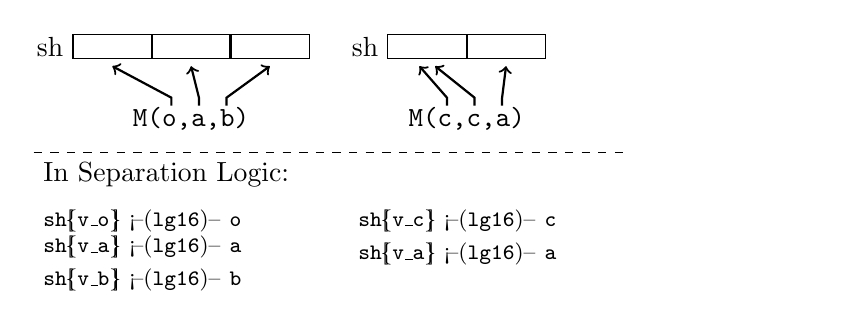
\begin{tikzpicture}
\def\-{\raisebox{.75pt}{-}}

\draw (0,0) rectangle (3,0.3);
\draw[thick] (1,0) -- (1,0.3);
\draw[thick] (2,0) -- (2,0.3);
\node [anchor=east] (shn) at (0,0.15) {sh};
\node [anchor=north] (Moab) at (1.5,-0.5) {\texttt{M(o,a,b)}};
\draw[thick, -> ] (1.25, -0.6) -- (1.25, -0.5) -- (0.5,-0.1);
\draw[thick, -> ] (1.6, -0.6) -- (1.6, -0.5) -- (1.5,-0.1);
\draw[thick, -> ] (1.95, -0.6) -- (1.95, -0.5) -- (2.5,-0.1);

\node [anchor=north west, text width=6cm, align=left] (Sepoab) at (-0.5,-1.8)
  {\footnotesize{$\mathtt{sh [\!\!\{ v\_o \}\!\!]\ \textrm{<\!--(}lg16\textrm{)--}\ o}$\\
  $\mathtt{sh [\!\!\{ v\_a \}\!\!]\ \textrm{<\!--(}lg16\textrm{)--}\ a}$\\
  $\mathtt{sh [\!\!\{ v\_b \}\!\!]\ \textrm{<\!--(}lg16\textrm{)--}\ b}$}};


\begin{scope}[yshift=0 cm,xshift=4 cm]
  \draw (0,0) rectangle (2,0.3);
  \draw[thick] (1,0) -- (1,0.3);
  % \draw[thick] (2,0) -- (2,0.3);
  \node [anchor=east] (shm) at (0,0.15) {sh};
  \node [anchor=north] (Mcaa) at (1,-0.5) {\texttt{M(c,c,a)}};
  \draw[thick, -> ] (0.75, -0.6) -- (0.75, -0.5) -- (0.4,-0.1);
  \draw[thick, -> ] (1.1, -0.6) -- (1.1, -0.5) -- (0.6,-0.1);
  \draw[thick, -> ] (1.45, -0.6) -- (1.45, -0.5) -- (1.5,-0.1);

  \node [anchor=north west, text width=6cm, align=left] (Sepoab) at (-0.5,-1.8)
    {\footnotesize{$\mathtt{sh [\!\!\{ v\_c \}\!\!]\ \textrm{<\!--(}lg16\textrm{)--}\ c}$\\
    $\mathtt{sh [\!\!\{ v\_a \}\!\!]\ \textrm{<\!--(}lg16\textrm{)--}\ a}$}};

\end{scope}

\draw[dashed] (-0.5,-1.2) -- +(7.5,0);
\node [anchor=north west] (sep) at (-0.5,-1.2) {In Separation Logic:};

\end{tikzpicture}
%
  \caption{Aliasing and Separation Logic}%
  \label{tikz:MemSame}%
\end{figure}

As a result, a function must either have multiple specifications or specify which
aliasing case is being used.
The first option would require us to do very similar proofs multiple times for a same function.
We chose the second approach: for functions with 3 arguments, named hereafter \texttt{o, a, b},
we define an additional parameter $k$ with values in $\{0,1,2,3\}$:
\begin{itemize}
  \item if $k=0$ then \texttt{o} and \texttt{a} are aliased.
  \item if $k=1$ then \texttt{o} and \texttt{b} are aliased.
  \item if $k=2$ then \texttt{a} and \texttt{b} are aliased.
  \item else there is no aliasing.
\end{itemize}
In the proof of our specification, we do a case analysis over $k$ when needed.
This solution does not cover all cases (\eg all arguments are aliased) but it
is enough for our needs.
